\documentclass[10pt]{article}
\usepackage{icmlko}

\icmlmeta{IP 파운데이션 월드모델}{183}{판이 숨기는 것을 보는 가드}{노트 182에서 판이 오르는데 팝업이 반 토막 났고 가드 열둘이 다 통과했다. 가드 열셋을 만들었다 --- 그리고 판이 왜 그걸 못 보는지가 산수로 나온다}

\begin{document}

\twocolumn[
\icmlheader

\begin{abstract}
노트 182가 시드는 축을 끄는 실험에서 판이 $+$0.0069 올랐는데 팝업이
0.343에서 0.127로 \textbf{반 토막}났고 \textbf{가드 열둘이 전부 통과}했다
--- 팝업은 손 축 다섯을 다 갖고 있어 맨몸도 안 걸린다. 그 실패 방식을 잡는
가드를 만들었다. \textbf{그늘}은 바꾸기 전 자료를 견주어 도메인마다 유보
$\rho$ 를 재고, 어느 하나가 0.10 넘게 내려가면 막는다. 알려진 네 경우에
대 봤다: 자기 자신과 견주면 전 도메인 낙차가 \textbf{정확히 0.0}이고(가드가
잡음을 안 만든다), 웹툰 두 축만 끄는 것은 \textbf{통과}하며(제일 나쁜
것이 아이돌 $-$0.037), 만화 · 세계애니를 끄는 것은 \textbf{막힌다}(세계애니
$-$0.104 --- \emph{자기 축을 끄고 자기가 손해 본다}), 전부 끄는 것도
\textbf{막힌다}(팝업 $-$0.148). 그리고 판이 왜 이걸 못 보는지가 산수로
나온다. \textbf{팝업은 유보 59건으로 판의 2.3\%다} --- $-$0.215 가
$-$0.005 로 줄어든다. 반면 게임은 8.6\%라 $+$0.119 가 $+$0.010 이 되고,
웹툰은 27.3\%라 $+$0.028 만으로 $+$0.008 을 낸다. \textbf{판은 크기 가중
평균이라 작은 도메인이 무너지는 것을 구조적으로 숨긴다} --- 웹툰과 애니
둘이 판의 50.5\%이고 팝업 · 아이돌 · 펀딩 셋을 합쳐야 6.4\%다.
\textbf{순위를 판 $\rho$ 로 정한다는 이 실험실의 첫 결정이 여기서 대가를
치른다.} 가드로 막는 것이 그 대가를 없애지는 않는다 --- 다만 대가를
치르고 있다는 것을 알려 준다. 마지막으로 한계를 적어 둔다: \textbf{그늘은
유보 라벨을 본다.} 거부권으로만 쓰고 고르는 데 쓰면 엿보기다 --- 무거운
가드 여덟이 이미 같은 성질이다.
\end{abstract}
]

\begin{figure*}[t]
\centering
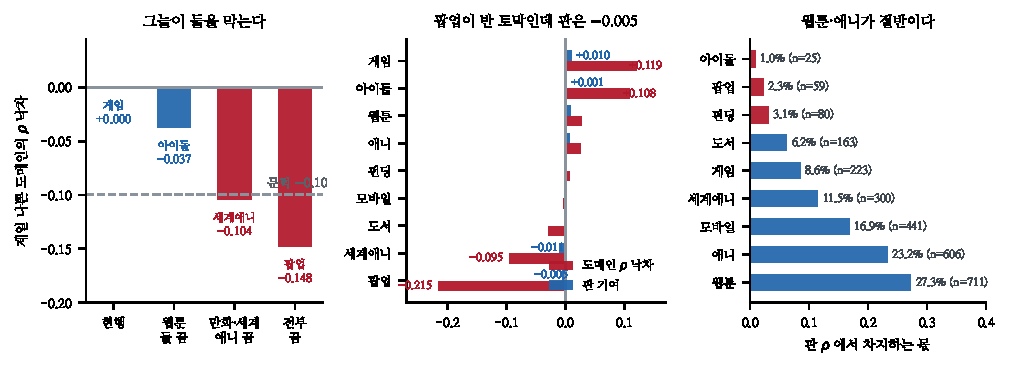
\includegraphics[width=\textwidth]{figs/shade.pdf}
\caption{왼쪽 --- 그늘이 둘을 막는다. 가운데 --- 팝업이 반 토막인데 판은
$-$0.005. 오른쪽 --- 웹툰 · 애니가 절반이다.}
\end{figure*}

\section{가드 열셋 --- 그늘}

\claimx{\textbf{무엇을 보나.} 바꾸기 전 자료(대개 기본 축만 실은 판)와
견주어 도메인마다 유보 $\rho$ 를 재고, 어느 하나가 문턱보다 크게 내려가면
막는다. 문턱은 0.10 으로 뒀다.}{기존 열둘은 전부 \emph{한} 실행 안의
성질을 본다 --- 엿보기 · 치환 · 재현 · 분모 · 빈칸 · 양규약 · 묶음 · 평탄
· 분해능 · 집단 · 시점 · 귀착 · 맨몸. \textbf{그늘만 두 실행을 견준다.}}

\begin{table}[t]
\centering\tsize
\caption{알려진 네 경우.}
\begin{tabular}{llrl}
\toprule
& 제일 나쁜 & 낙차 & \\
\midrule
현행(자기 비교) & --- & \textbf{0.000} & 통과 \\
\textbf{웹툰 둘 끔} & 아이돌 & $-$.037 & \textbf{통과} \\
만화·세계애니 끔 & 세계애니 & $-$.104 & \textbf{막힘} \\
전부 끔 & 팝업 & $-$.148 & \textbf{막힘} \\
\bottomrule
\end{tabular}
\end{table}

\claimx{\textbf{자기 비교가 정확히 0 이다} --- 아홉 도메인 전부. 가드가
잡음을 안 만든다는 귀무 확인이다.}{씨앗을 고정하고 같은 적합을 두 번 하는
것이라 당연해 보이지만, 노트 146에서 F18 이 씨앗에 팝업 $\rho$ 0.059
움직인 것을 봤다. \textbf{확인할 값이 있었다.}}

\claimx{\textbf{세계애니가 자기 축을 끄고 자기가 손해 본다}($-$0.104).
만화 · 세계애니의 손 축 셋씩을 끈 실험인데, 세계애니 자신이 제일 크게
잃고 게임이 $+$0.124 얻는다.}{\textbf{순이득이 아니라 재배분이다} ---
풀링 계수가 만화 · 세계애니에서 게임 쪽으로 옮겨 간다. 판만 보면 $+$0.0069
로 ``좋아졌다''고 읽힌다.}

\section{판이 왜 못 보나}

\begin{table}[t]
\centering\tsize
\caption{도메인 낙차와 판 기여. 전부 끔.}
\begin{tabular}{lrrrr}
\toprule
& 유보 n & 몫 & 낙차 & 판 기여 \\
\midrule
\textbf{팝업} & 59 & \textbf{2.3\%} & \textbf{$-$.215} & \textbf{$-$.0049} \\
게임 & 223 & 8.6\% & $+$.119 & $+$.0102 \\
\textbf{아이돌} & 25 & \textbf{1.0\%} & $+$.109 & $+$.0010 \\
세계애니 & 300 & 11.5\% & $-$.095 & $-$.0110 \\
\textbf{웹툰} & 711 & \textbf{27.3\%} & $+$.028 & \textbf{$+$.0075} \\
애니 & 606 & 23.2\% & $+$.026 & $+$.0061 \\
\midrule
합 & 2608 & 100\% & & $+$.0069 \\
\bottomrule
\end{tabular}
\end{table}

\claimx{\textbf{팝업이 반 토막 나도 판은 0.005 내려간다.} 아이돌이 0.109
올라도 0.001 오른다. 반면 웹툰은 0.028 만 올라도 0.008 을 낸다.}{크기
가중이 그렇게 만든다 --- 웹툰과 애니 둘이 50.5\%이고 팝업 · 아이돌 · 펀딩
셋을 합쳐야 6.4\%다. \textbf{작은 도메인은 무슨 일이 나든 판에 안 보인다.}}

\claimx{\textbf{이건 판정치의 성질이지 잘못이 아니다.} 노트 82 · 90에서
분모를 정할 때 크기 가중을 고른 까닭이 있었다 --- 표본 스물다섯짜리
도메인의 $\rho$ 는 오차가 커서 같은 무게를 주면 잡음이 순위를
흔든다.}{\textbf{그래도 대가는 있다} --- 팝업은 이 프로젝트의 출발점이고
(노트 1$\sim$130) 지금은 판의 2.3\%다. \textbf{순위를 판 $\rho$ 로
정한다는 첫 결정이 여기서 값을 치른다.}}

\claimx{\textbf{가드가 대가를 없애지는 않는다.} 그늘은 큰 낙차를 알려 줄
뿐 판정치를 안 바꾼다.}{바꾸는 방법도 있다 --- 도메인 균등 가중이나 최소
도메인 $\rho$ 를 같이 적는 것. \textbf{판정치를 바꾸는 것은 이 노트에서
안 한다} --- 노트 82의 분모 규칙대로 자료가 아니라 점수를 보고 바꾸는
것이 되기 때문이다.}

\section{한계}

\claimx{\textbf{그늘은 유보 라벨을 본다.} 그래서 \emph{거부권}으로만 쓴다
--- 여러 후보를 그늘로 걸러 제일 좋은 것을 고르면 그건 엿보기다.}{무거운
가드 여덟(엿보기 · 치환 · 재현 · 묶음 · 평탄 · 분해능 · 집단 · 귀착)이
이미 같은 성질이다. \textbf{가드는 참을 주장하는 도구가 아니라 거짓을
막는 도구다.}}

\claimx{\textbf{문턱 0.10 은 근거가 약하다.} 노트 182의 낙차 분포에서
$-$0.104 와 $-$0.037 사이에 그은 것이다.}{노트 152의 검출 한계로 보면
표본 스물다섯짜리 아이돌은 짝 반폭이 0.2 를 넘으므로 0.10 문턱이 그
도메인에서는 잡음에 걸릴 수 있다. \textbf{표본별 문턱이 맞겠지만 안
했다.}}

\begin{table}[t]
\centering\tsize
\caption{남은 것.}
\begin{tabular}{ll}
\toprule
\textbf{문턱} & 표본 크기에 따라 달라야 한다 \\
판정치 & 최소 도메인 $\rho$ 를 나란히 적을 것인가 \\
팝업 & 판의 2.3\% --- 출발점이 사라지고 있다 \\
\bottomrule
\end{tabular}
\end{table}

마지막 줄이 이 흐름에서 제일 크다. 이 실험실은 팝업 하나로 시작했고
(노트 1$\sim$130) 도메인을 열까지 늘리면서 판 $\rho$ 를 순위로 세웠다.
그 결과 \textbf{팝업에 무슨 일이 나든 순위가 안 바뀐다.} 노트 130까지
쌓은 팝업 지식이 지금 판을 못 움직인다는 뜻이고, 그것이 좋은 일인지
나쁜 일인지는 이 판으로 못 정한다 --- \textbf{IP 파운데이션 월드모델이
무엇을 하는 물건이냐에 달렸다.}

\end{document}
